% !TeX root = document.tex
% !TeX encoding = UTF-8 Unicode

\chapter{Practical Implementation Aspects}%
\label{chp:practival-implementation-aspects}

When implementing the techniques described in this thesis, some details need
attention. For example, it is easy to say
\enquote{\(\mathrm{minimize}~f(x)~|~x\in\mathcal{X}\)}, however it is not so
simple (and sometimes even possible) to implement the \(x\in\mathcal{X}\) bit.
Describing the set and finding a way to test membership numerically can be
challenging. That is one reason why we choose convex sets: we know how to
implement membership tests and use it in common optimization frameworks.

This chapter will discuss how to represent the constraints and region of
attraction and provide some insight into how to implement the models of the
command governor with a supervisor structure, the problems faced when resetting
integrators and estimating the region of attraction.

\section{Polytope representations}%
\label{sec:polytope-representation}

A convex polytope can approximate any convex region. A convex polytope is a
compact convex set with a finite number of extreme points such that, for any two
distinct points \((a,b)\) belonging to the region, a closed segment with
endpoints \((a,b)\) is entirely contained within the
region~\parencite{grünbaum:convex}. In other words, it is a convex hull of a
finite number of points, called vertices. This representation is called the
\enquote{V-representation} and is not useful to test membership. However, it is
straightforward to sample points from the desired region's border to create a
V-representation of a polytope approximating it. It is also useful for plotting.
The Figure~\ref{fig:v-rep-example} illustrates a region in its V-representation,
where the red dots are the vertices, and all blue dots are inside the region.
The set of vertices is \resizebox{\linewidth}{!}{%
\(\{(0.02,0.71),(0.31,0.02),(0.82,0.04),(0.87,0.13),(0.99,0.88),(0.60,0.98),(0.38,0.97),(0.04,0.88),(0.02,0.82)\}\)}.

\begin{figure}[!htb]
	\centering
	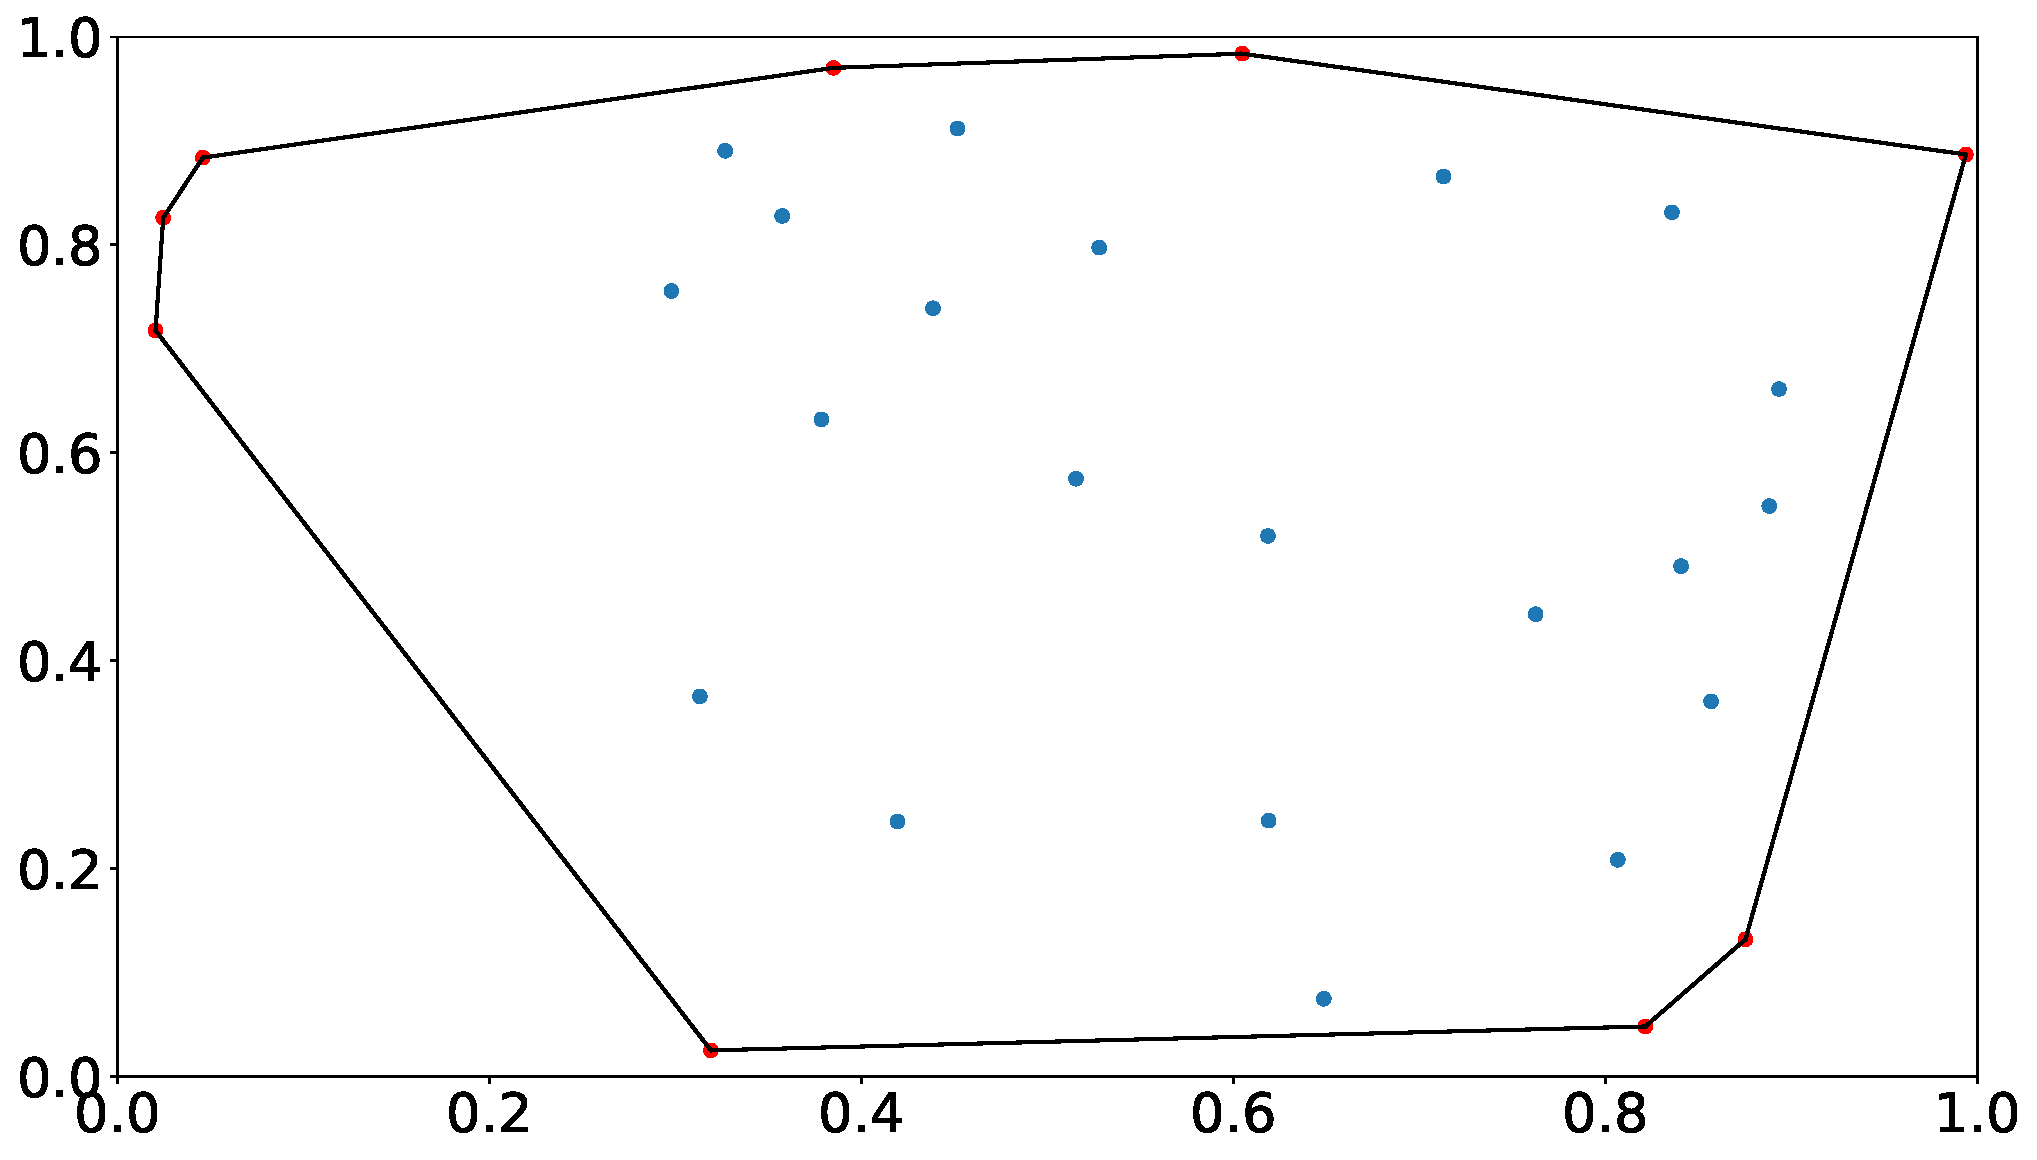
\includegraphics[width=\linewidth]{imgs/v-rep}
	\caption{Visualization of the V-representation of a set}%
	\label{fig:v-rep-example}
\end{figure}

A more useful representation of such regions is the \enquote{H-representation}.
In this representation, the intersection of a finite number of half-spaces
describes the region. A half-space is one of the two parts in which a
hyper-plane divides an affine space. Since half-spaces are linear inequalities,
the H-representation becomes the matrix inequality
%
\begin{equation}
	Ax\leq{}b,
\end{equation}
%
where \(A\) is a matrix of coefficients, \(x\) is a point in space and \(b\) is
a vector of real numbers. The number of rows in \(A\) and \(b\) is the same as
the number of half-spaces defining the region. All points satisfying the
inequality are in the region's interior, making it easy to test set membership.
Figure~\ref{fig:h-rep-example} shows the half-spaces that compose the
H-representation of the same convex polytope presented in
Figure~\ref{fig:v-rep-example}. Equation~\ref{eq:h-rep-example} shows the
inequation that describes the region. The selected side is not shown for each
half-space but is the one in which intersections with the other selected halves
make the convex region in the middle.

\begin{equation}
	\label{eq:h-rep-example}
	\begin{bmatrix}
		-0.91 & -0.39 \\
		0.04  & -0.99 \\
		0.98  & -0.15 \\
		0.84  & -0.54 \\
		-0.24 & 0.96  \\
		0.24  & 0.97  \\
		-0.06 & 0.99  \\
		-0.99 & 0.03  \\
		-0.93 & 0.34
	\end{bmatrix}x \leq
	\begin{bmatrix}
		-0.30 \\
		-0.01 \\
		0.84  \\
		0.66  \\
		0.84  \\
		1.10  \\
		0.94  \\
		0.00  \\
		0.26
	\end{bmatrix}
\end{equation}

\begin{figure}[!htb]
	\centering
	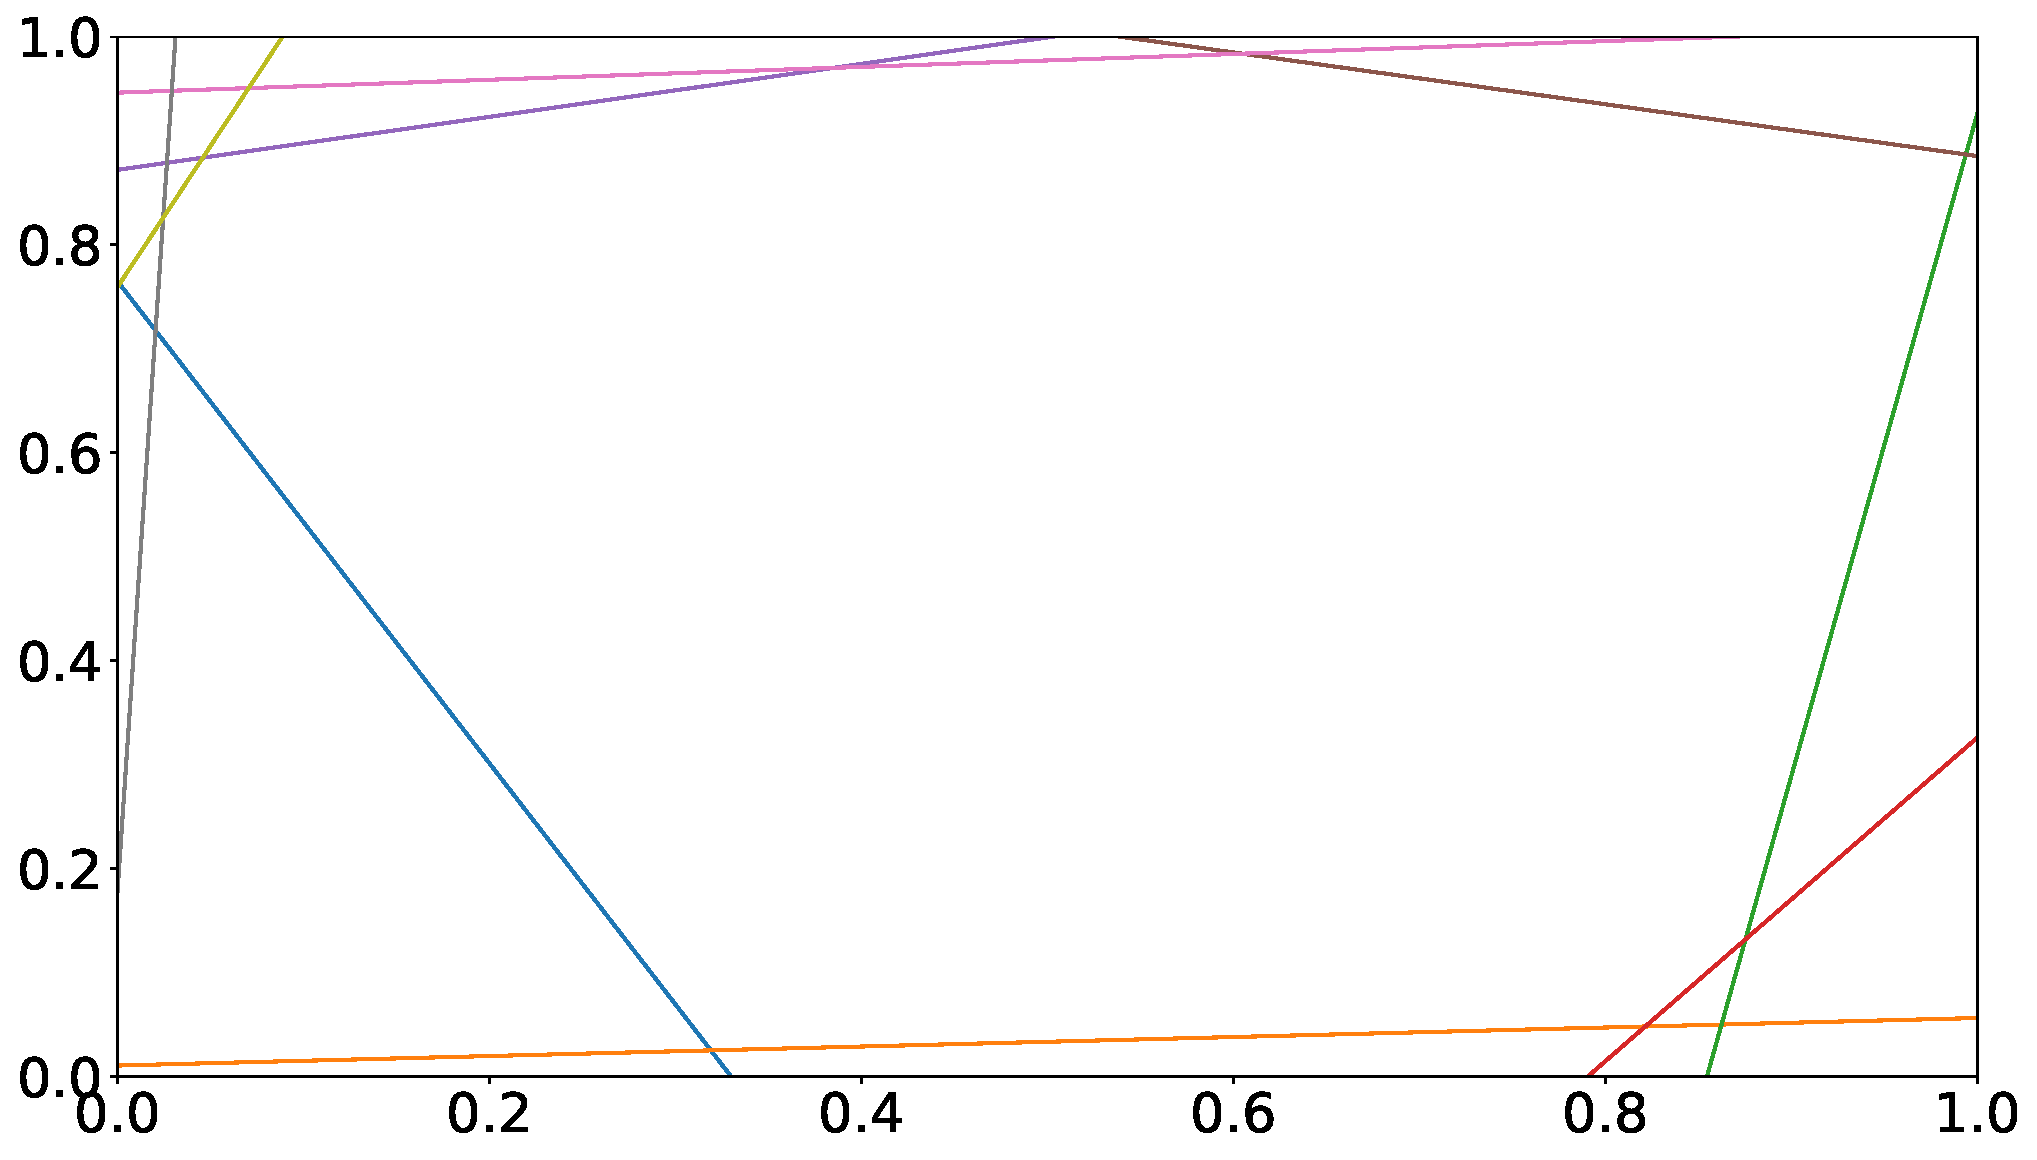
\includegraphics[width=\linewidth]{imgs/h-rep}
	\caption{Visualization of the H-representation of a set}%
	\label{fig:h-rep-example}
\end{figure}

Given that the V-representation is easier to obtain from generic shapes, but the
H-representation is more useful when verifying set membership, it is essential
to have a way to switch between them. Unfortunately, this is not
straightforward, but some algorithms allow us to enumerate the facets given the
vertices. Some problems of such algorithms are the time needed to find the
facets of many vertices and how to find facets in higher-order spaces. However,
good algorithms can be used for the conversion, especially if the computation
will be offline
\parencite{avis.bremner.ea:how,graham.frances-yao:finding,lee:on,mccallum.avis:linear}.

Particular regions can be easily described in a way that is easy to include in
optimization problems. The ellipsoid is one such region, as it is described as
\(x^{T}Px\leq{}1\) so that any point \(x\) that satisfies the inequality is inside
the region. Any region described by polynomials can be expressed in a matrix
form and can quickly test membership. Such regions should use their inequation
directly instead of a polytope approximation.  We do that to the Region of
Attraction, and it is how we implemented the check to verify if the state is
inside it.

\section{Internal Models}%
\label{sec:internal-models}

To switch modes and controllers of a system the way we propose, one must pay
attention to the controller's internal states and the control signal's
continuity. Also, since every CG unit has its controller and model, the
destination CG must be updated to a valid state before switching. There are many
ways to do so, and we will present some.

Probably the best way is to run all CGs in parallel. The optimization problem of
the inactive units does not need to run with complete constraints. It can be
relaxed only to contain the region constraint on the virtual reference; also,
the observer can be ignored. It is necessary to find the virtual reference,
which will be close to the constraint region's border, which is closest to the
real system's state. Notice that, in this case, we are not looking for a virtual
reference closest to the real reference but to the real system's state. By doing
so, the internal model's and the controller's states will always be valid.

However, this approach can be resource-intensive, as it still computes the
optimization problem at every sample. It is also possible to run the observer
and update the internal model's states without checking for constraint
violations, but this does not solve the controller's state problem. Another
technique needs to be combined to find them.

Another way of guaranteeing valid states is to compute the states before
changing mode. Two ways of computing the states are: by inverting the system and
controller equations and by simulation. The first approach has a very low
computational resource impact but may not be possible or yield not ideal values.
For systems with integrators, for example, there will be infinitely many
results. Another problem is that even though the system has only one
steady-state solution, it can have many transient ones.

The simulation becomes interesting, even though it is more computationally
intensive, as it can calculate a state that better matches the current
transitory characteristics of the real system. It can also find the model's and
controller's states at once, guaranteeing that there is no mismatch. To use the
simulation approach, execute the simulation right before changing modes, using
the internal controller and model, and setting the reference to the real
system's current state. This yields a valid steady-state model's and
controller's state. However, this technique does not guarantee control signal
continuity without adjustments.

\section{Integrator Reset}%
\label{sec:integrator-reset}

Integrator Reset

\section{Region of Attraction Estimation}%
\label{sec:roa-estimation}

Region of Attraction Estimation
